\section{Energy Demand and Supply}
At the basis of our work is the knowledge of a realistic energy demand profile, that would catch the transients throughout the year.
Given our focus on the residential sector, the overall energy demand can be seen as the sum of the heating/cooling contribution + all the other electricity consuptions for appliances and lightning.
Several semplifications will be made through the following derivation but we point out any possible improvment that could be made but was considered out of the scope of this work.

\subsection{Approach}
\subsubsection{Introduction}
In Italy, an APE (Attestato di Prestazione Energetica) is a document that certifies the energy performance of a propriety unit (unità immobiliare). This certification must be issued by a qualified technician and is mandatory for all buildings that are sold, rented or refurbished. 

The APE provides information about the energy consumption of the property, its energy class. The energy class is a letter grade (from A4 to G) that indicates the energy performance of the building, with A4 being the most efficient and G being the least efficient.

Each unit refers to a distinct and identifiable part of a real estate property, such as an apartment, a house, or a commercial space, that can be individually owned, sold, or rented. It is a specific segment of a larger property that has its own legal and functional identity. For instance, a building with three apartments will have three separate APEs, one for each apartment.
For this reason we can safely assume that each unit is the residence of a single family.

\subsubsection{Methodology}
We plan to determine the demand profile of electricity in the region $P_{e, \text{tot}}$.

From simulations we are able to retrive the hourly demand profile of thermal energy for heating $\dot{Q}_h$ and cooling $\dot{Q}_c$ for each energy class $i$.
This is converted to electicty demand by taking into account the share of buildings in that energy class that use a heat pump for climatization purposes $\text{\chi}_{HP}$ and its efficency for heating $COP$ and for cooling $EER$. To this we then add a contribution of electric consumption for other purposes $P_{other}$.

\begin{equation}
    P_{e,i}^- = 
    \left( 
        \frac{\dot{Q}_{h,i}}{COP} 
        + 
        \frac{\dot{Q}_{c,i}}{EER} 
    \right)  
    \cdot 
    \text{\chi}_{HP} 
    + P_{other}
\end{equation}

Then we estimate the production of photovoltaic systems for each energy class $P_{e,i}^+$. Finally the reference energy demand for each energy class can be obtained by subtraction of demand and production: $P_{e, \text{ref}, i} = P_{e,i}^- - P_{e,i}^+$

Then, we can simply sum the contributions, each wheighted on their respective class share $\text{\chi}_{i}$, to get a reference profile of the region under study.
This can be multiplied by the number of buildings in the region $N_{\text{UI}}$ to obtain the total demand $P_{e, \text{tot}}$.

\begin{equation}
    P_{e, \text{tot}} = 
    N_{\text{UI}} 
    \cdot 
    \sum_{i=\text{A4}}^{\text{G}} P_{e, \text{ref}, i} 
    \cdot 
    \text{\chi}_{i} 
\end{equation}



\subsubsection{Data Sources}
From the CENED database \cite{cened2025} we extracted the information about the relevant municipalities of the region,
which we derived based on the map of primary substations from the national grid operator (GSE) \cite{gse_cabine_primarie}.
The data was also filtered to include only residential buildings, excluding commercial and industrial ones.
This was necessary given the large amount of data from the complete regional database. This way an easier to manage csv file was obtained.
Note that an API is available to access the database but it was found to be very slow and inefficient.

\subsection{Heating and Cooling Demand}
For each energy class we have taken a real example of a residential building from the region under study and computed the 
hourly thermal demand for heating and cooling thoughout the year.
This is obtained by means of a professional software (TERMOLOG) that allows for dynamic simulation of the energy system of the building.
This computation is based on the UNI EN ISO 52016 standard.
We used one reference building per energy class all with the same utlization profile, which is a simplification to be discussed later.
The output of the calculation is an hourly profile of the thermal demand for heating and cooling.

% Add one example of the houdly profile

\subsubsection{Normalization of the Data}
The data of each building had to be normilized to be rapresentative of the "average building".
To do so we used the "userful heated area" information from the CENED database.
This is the area of the building that is actually used for heating and cooling, excluding areas such as garages, attics, and basements.
We normalized the reference profiles over their area and then used the average area 
of the buildings removing the top 99 buildings since some anomalies have been encountered.
The average area ended up being $91.37 m^2$.

\begin{figure}[H]
    \centering
    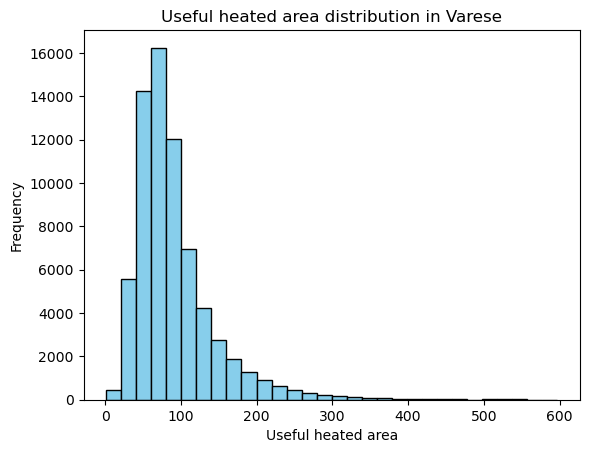
\includegraphics[width=0.8\textwidth]{figures/1_building_area_histogram.png}
    \caption{Histogram of the useful heated area of buildings.}
    \label{fig:building_area_histogram}
\end{figure}

\subsection{By class distributions}
To be able to simply simulate different scenarios we have identified characteristics of each energy class 
so that we can just modify the energy calss distribution and all the parameters needed to determine the energy demand will follow.

\subsubsection{Heat Pump distribution and Cooling Demand}
We identified the share of heat pumps per energy class.
We also determined the share of buildings that have a cooling system installed, which as of today comes up to $9.58\%$. 
This is a very low share and is to be expected as the region under investigation is quite chill during summer.

\begin{figure}[H]
    \centering
    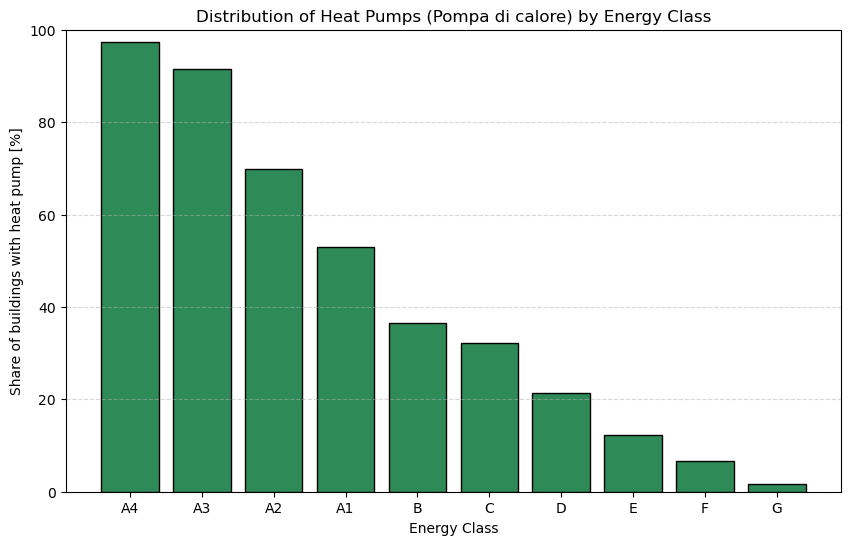
\includegraphics[width=0.8\textwidth]{figures/1_heat_pump_distribution.png}
    \caption{Distribution of heat pumps across energy classes.}
    \label{fig:heat_pump_distribution}
\end{figure}

\subsubsection{Photovoltaic Distribution}
We identified the share of building that have photovoltaic systems installed per energy class.
\begin{figure}[H]
    \centering
    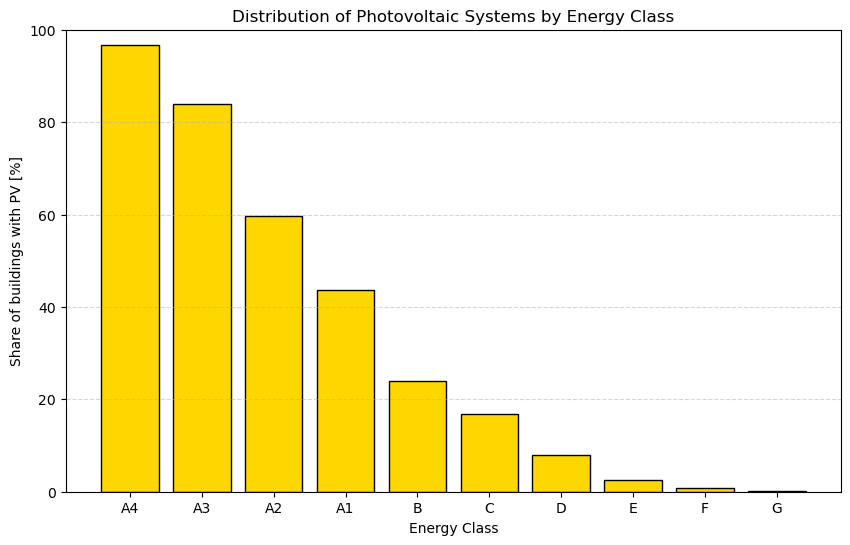
\includegraphics[width=0.8\textwidth]{figures/1_photovoltaic_distribution.png}
    \caption{Distribution of photovoltaic systems across energy classes.}
    \label{fig:pv_distribution}
\end{figure}

Moreover we then divided the data into two groups, those with an heat pump and those without.
From these we plotted the distribution of the size of the photovoltaic system installed. And computed the average (of the $P_99$)

\begin{figure}[H]
    \centering
    \begin{subfigure}[b]{0.45\textwidth}
        \centering
        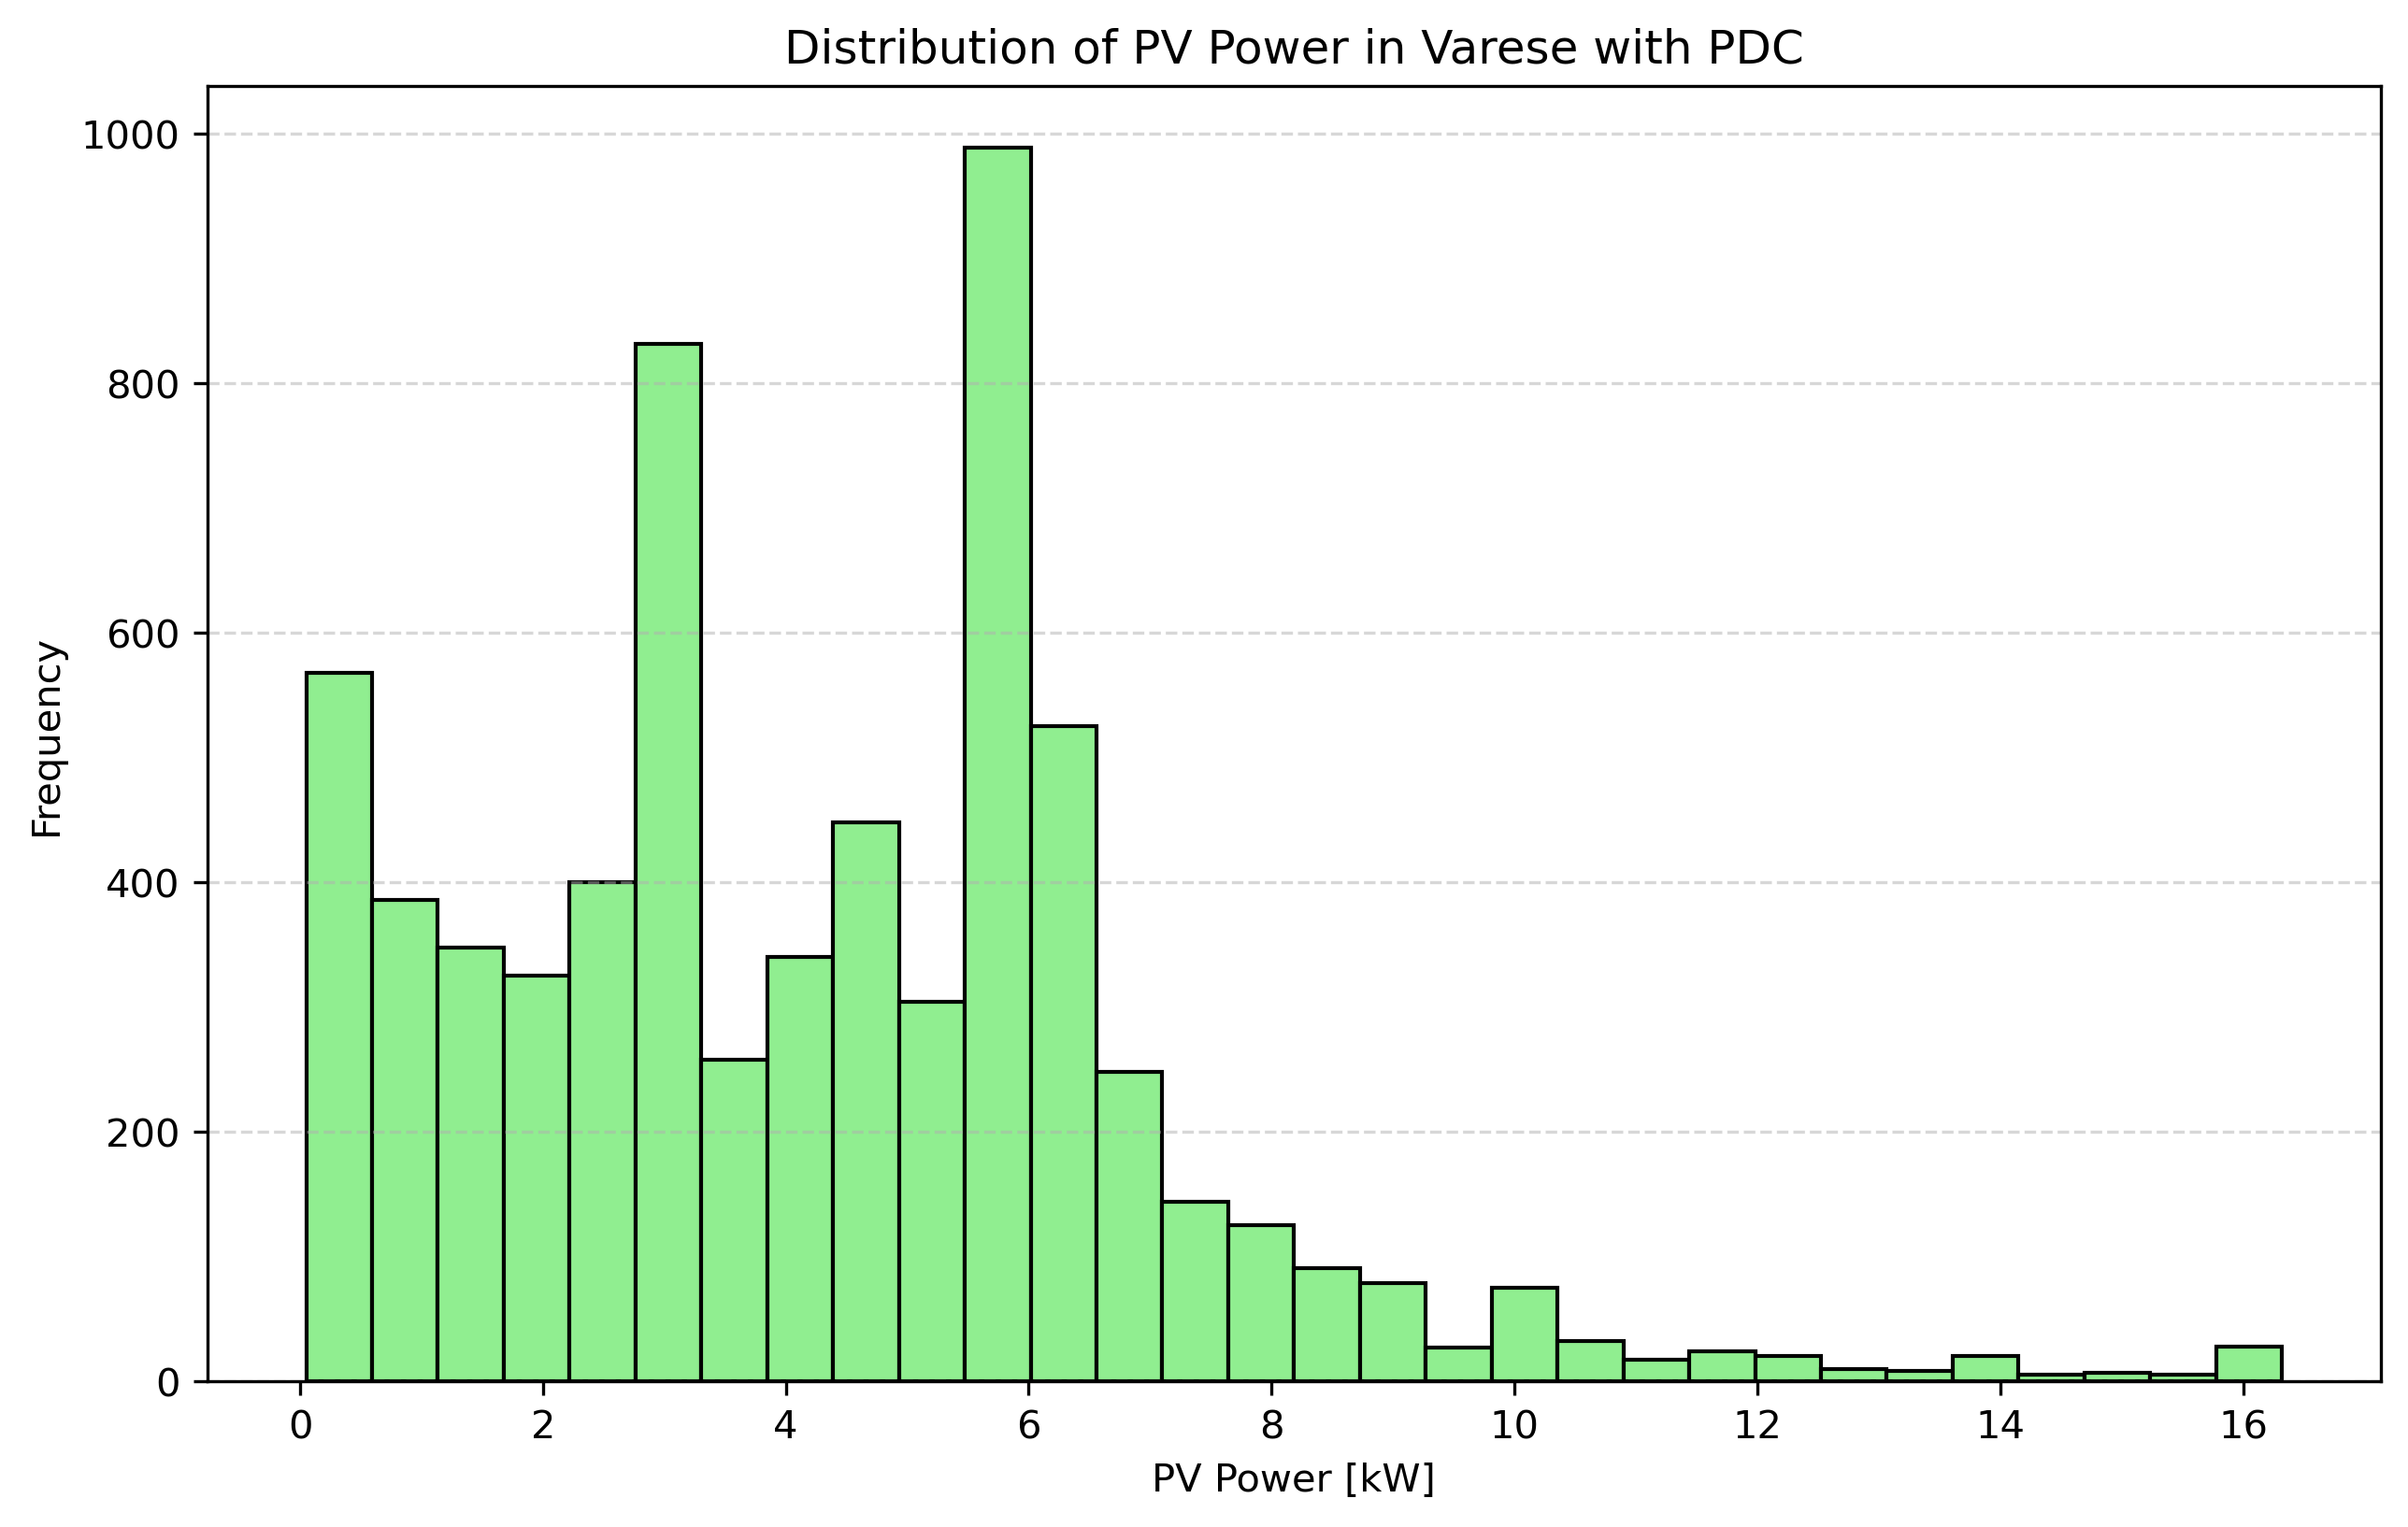
\includegraphics[width=\textwidth]{figures/1_pv_size_hp.png}
        \caption{Photovoltaic system size distribution for buildings with heat pumps.}
        \label{fig:pv_size_hp}
    \end{subfigure}
    \hfill
    \begin{subfigure}[b]{0.45\textwidth}
        \centering
        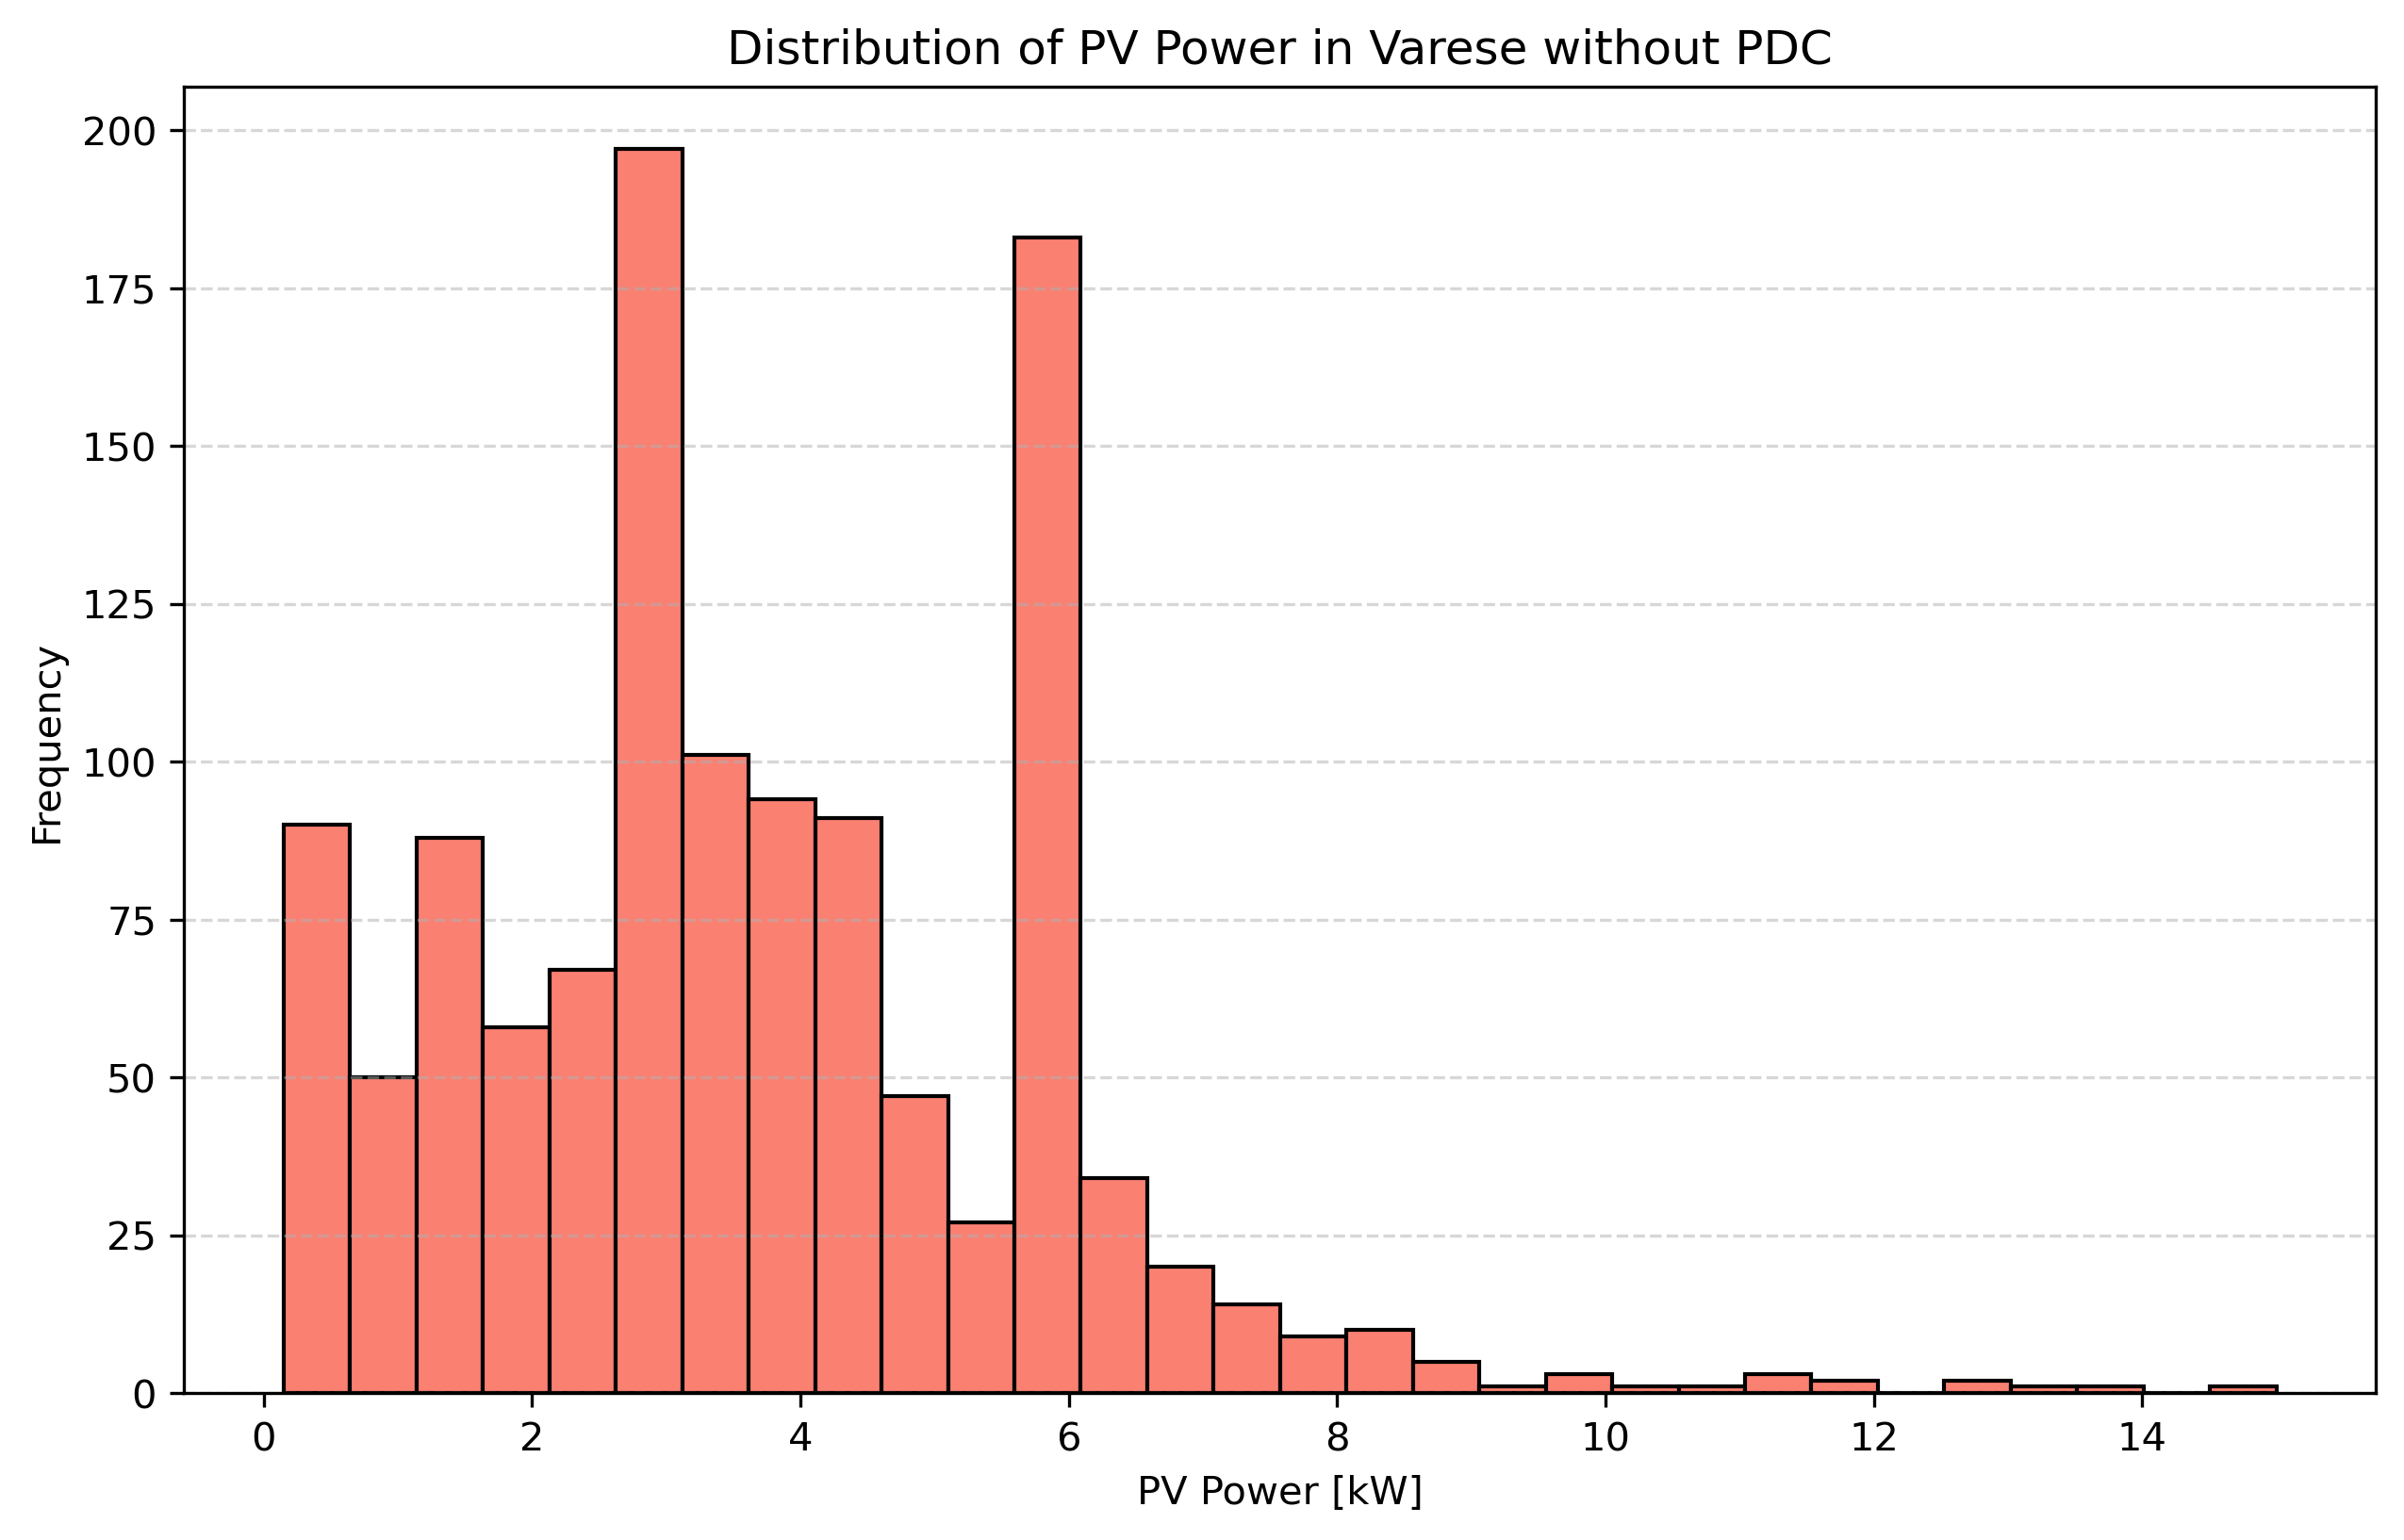
\includegraphics[width=\textwidth]{figures/1_pv_size_no_hp.png}
        \caption{Photovoltaic system size distribution for buildings without heat pumps.}
        \label{fig:pv_size_no_hp}
    \end{subfigure}
    \caption{Distribution of photovoltaic system sizes based on heat pump presence.}
    \label{fig:pv_size_comparison}
\end{figure}

The averages values are: $4.30$kW and $3.70$kW for the sistem with and without heat pumps respectevely.

\paragraph{Observation on the relative sizes of PV systems}

Another interesting information we gathered is the relative size of the photovoltaic system. 
Using data from the CENED database: Exported Electricity, Imported Electricity and In situ consumption.

\begin{equation}
    \text{SCF: Self-Consumption Factor} = \frac{\text{In situ consumption}}{\text{Import} + \text{In situ consumption}}
\end{equation}

\begin{equation}
    \text{OSF: Over-Sizing Factor} = \frac{\text{Export - Import}}{\text{Import} + \text{In situ consumption}}
\end{equation}

Whie the SCF is quite obvius, 
we defined the OSF to consider the resonable oversizing of the system that ensures that the energy exoported covers, at least, the imported energy.
A value of $0\%$ indicates a balanced system, positive values indicate greater export then import, negative the opposite.

\begin{table}[H]
    \centering
    \begin{tabular}{|c|c|c|}
        \hline
        \textbf{Class} & \textbf{SCF (\%)} & \textbf{OSF (\%)} \\
        \hline
        A4 & 38.49 & 65.47 \\
        A3 & 55.92 & 78.28 \\
        A2 & 68.32 & 299.50 \\
        A1 & 74.43 & 1029.90 \\
        B  & 80.71 & 966.47 \\
        C  & 84.49 & 434.58 \\
        D  & 90.84 & 111.82 \\
        E  & 96.08 & 120.58 \\
        F  & 98.85 & -67.53 \\
        G  & 99.76 & -95.48 \\
        \hline
    \end{tabular}
    \caption{SCF and OSF indicators by Energy Class.}
    \label{tab:pv_scf_osf}
\end{table}

The extreme overdimensioning on some classes can be explained as the result of two effects:
\begin{itemize}
    \item Units with PV installed but using gas for heating.
    \item Simplified calculation of the CENED engine
    \item Counter effects of inventives and tax deductions.
\end{itemize}

Units in the middle of the energy class scale (A1 to D) are likely to still use gas for heating, as seen from the previous Figure~\ref{fig:heat_pump_distribution}.
None the less a some of them still have a photovoltaic system installed. This means that most of the energy produced is not used on site.

Regarding the CENED engine, it is important to note that is uses a simplifyued calculation: it computes monthly averages, doesn't take into account energy storage,
nor it consider any other time of electric consumption (such as appliances or lighting).

At last, it's known from professional experience that boost the energy class,
it is common that contractors choose to an over sized photovoltaic system. 
This practice was particularly common during the "superbonus" (2020-2023) period which required a mandatory jump of 2 energy classes to be eligible for the tax deduction.
It could be interesting to evaluate the impact of this on the efficiency of the grid.

\subsubsection{Electricity Production}
We have to obtain a reference value of the photovoltaic production profile.
First, the list of municipalities is fed to the Nominatim API \cite{Nominatim} to obtain the coordinates of the center of each municipality.
Then, we use the PVGIS API \cite{PVGIS} to obtain the hourly production profile for each municipality.
We fixed the angle to an average $22^\circ$ and a plant size of $1kW$.
For each municipaly we obtain a profile every $10^\circ$ of the azithmut angle, from $0^\circ$ to $360^\circ$. 
Those are then weighted to a gaussian distribution to represent that it is prefered to point the photovoltaic system to the south.
This gives us a reference photovoltaic production profile for each municipality $P_{e,m}^+$, where $m$ is the municipality.
Then we can obtain the reference production profile for each energy class $P_{e,ref}^+$ by weighting the production profile of each municipality on the share of buildings in that municipality over the total.

Finally to obtain the referece production profile we used the following formula:
\begin{equation}
    P_{e}^+ 
    = 
    \sum_{i=A4}^{G}
    P_{e,ref}^+ 
    \cdot 
    \left( 4.30 \chi_{hp}(i) + 3.70 (1-\chi_{hp}(i)) \right)
    \cdot
    N_{b}(i) \chi_{pv}(i)
\end{equation}


\subsection{Convertion from thermal to primary energy demand}
The dynamic simulation outputs the thermal demand of the building. 
To estimate the primary energy needed we used average efficiencies of the heating and cooling systems.

\begin{equation}
    \dot{Q}_{\text{fossil}} = \frac{\dot{Q}_{\text{th}}}{\eta_{\text{fossil}}}
\end{equation}

\begin{equation}
    P_e = \frac{P_{\text{th, heating}}}{\text{COP}_{h}} + \frac{P_{\text{th, cooling}}}{\text{COP}_{c}}
\end{equation}

\subsection{Other Electricity Demand}
% Once we settle on the numbers report them here
Electrical demand for appliances and lighting is modeled equal for all classes.
The definition was manual, hour by hour for an average day in the following "seasons":
\begin{itemize}
    \item Winter Weekday
    \item Winter Weekend
    \item Summer Weekday
    \item Summer Weekend
    \item Winter Holiday
    \item Summer Holiday
\end{itemize}
Moreover we added an absence factor to take into account when people go on holiday massively during august.

The profile is defined by considering the following contributions:
\begin{itemize}
    \item standby and always on appliances
    \item lighting 
    \item appliances
\end{itemize}
During the summer the need for a cooling fan was added.  
Moreover we added a parameter to rapresent the share of buildings with an induction system installed.

% reference hourly profile through the year

\subsection{Total Grid Demand}
In the end we choose an energy class distribution to rapresent a future scenario.
Given that we know the reference demand-production profile of each building we can sum them up by  weighting on their supposed share to obtain the total reference demand
which is then multiplied by the number of buildings in the region to obtain the total demand.

% WIP how many buildings in the region

\subsubsection{Comparison and Tuning}
To verify our method is acceptable we compare the total demand by the data available online, in particual we compared it to the average annual deamnd,
in the residential sector for the province of Varese \cite{portaleconsumi_energia_domestica}, which happends to be $1931 kWh$ in 2023,
with a decreasing trend in the last years ($2016kWh$ in 2022 and $2119kWh$ in 2021). 

% WIP tuning the data

\subsubsection{Possible Improvments}
It is defenitly possible and could give better results if the data for each class was obtained by a set of real building from the region instead of just one.
Ideally one would use a statistically signfinicant set of buldings and vary the utilization profile as well.
Moreover, it would be beneficial to wheight the simulation data on the real energy requirments of those same buildings,
which is a much more complex task since it would require extensive data acquisition during the year. 
While this is feasible for electrical demand (most operators give to the customer a detailed bill with hourly consumption),
it is much more difficult to get the same data for fossil fuel consumption.
At last, the normalization has been done with the heated area an not with the volume (which is much more indicative of the energy requirment of a building) 
given the on-field knowledge that the volume is usually approximatly obtained by a the rule of thumb of multiplying the heated area by a factor of 2.7 or 3 in most cases.
From the simulation we have neglected humidification and dehumidification electricity needs since these plants are rearly installed today,
a better evaluation would evaluate the possible future share of air treatment plants in the residential sector.

Photovoltaic: We have neglected any solar-thermal system installed since their are considered not very impactful and their impact is complex to evaluate.

Convertion thermal to primary: use time dependent efficiency for heat pumps that take into account the ambient temperature,
this could be accomplished considering that our code uses hourly data.

Other Electricity Demand: This is without a doubt the most complex contribution to evaluate,
expecially considering that it is not easy to imagine how the electricity consumption will evolve in 25 years.
It could be improved by collecting a statistically signficant number of examples from the region on the type of appliances installed and their consumption.

Overall: the methodology of using class distribution as a way of evaluating the energy demand is considered a good approach,
for the best results we shall gather consumption data for both electric and fossil fuels for a statistically significant number of buildings for each energy class.